% Resultados Obtenidos. Bancos de medición según ISO10373, resultados, verificación de la lógica y conclusiones.
\chapter{Implementación, Evaluación y Resultados}

En este capítulo se verán los detalles concernientes a la 
implementación en silicio del circuito integrado y la integración de 
todos los bloques en un solo dispositivo. También se 
describirá el método de verificación utilizado y luego se verán las 
mediciones realizadas con sus resultados.

\section{\emph{Layout} Completo del Circuito Integrado}

El trazado físico (\emph{layout}) de los dispositivos y conexiones se 
realizó utilizando las herramientas de \emph{Mentor Graphics} 
\cite{MentorCustomIC} junto con el kit de diseño del proceso C5N entregado por 
MOSIS. El kit de diseño define el set de máscaras a utilizar por la 
herramienta para el trazado del \emph{layout} del circuito integrado y 
contiene las reglas del proceso con los tamaños y distancias mínimas 
entre máscaras. Además contiene una serie de dispositivos 
predefinidos como son transistores, resistores y capacitores. El 
esquemático está vinculado con el layout de forma tal que cada uno 
de esos dispositivos se coloca en el layout según los tamaños definidos 
en el esquemático. A esta forma de trabajo se la llama \emph{Schematic 
Driven Layout} (SDL) y fue la que se utilizó para el trazado de los 
dispositivos y el conexionado de los diferentes bloques.

El tamaño del \emph{die} provisto por MOSIS es de 
\(\SI{1500}{\micro\meter}\times\SI{1500}{\micro\meter}\), sin embargo 
el área disponible para el diseño fue la mitad, 
\(\SI{1500}{\micro\meter}\times\SI{750}{\micro\meter}\), ya que el chip 
fue compartido con otro proyecto. La biblioteca de celdas digitales de 
la \emph{Oklahoma State University} (OSU) \cite{OSUstandardCells}
contiene \emph{buffers} de entrada/salida cuyo layout está formado por 
un \emph{bond pad}\footnote{El área de metal donde se suelda la 
conexión al encapsulado} y protecciones contra descarga 
electrostática (ESD por sus siglas en inglés). Estos buffers se colocan 
en la periferia del chip formando un anillo alrededor del mismo de 
forma tal que los buffers quedan conectados entre si formando un 
\emph{bus} de alimentación. Estas estructuras fueron utilizadas para 
todas las entradas y salidas digitales, 17 en total, por lo que gran 
parte del área disponible fue ocupada con los buffers, como se observa 
en la figura \ref{fig:LayoutCompleto}.

\begin{figure}
	\centering
	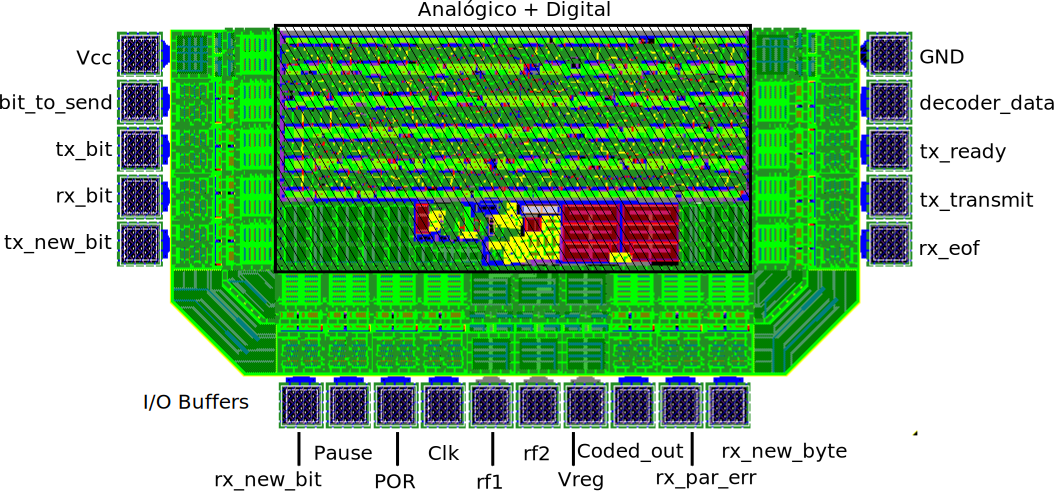
\includegraphics[width=\linewidth]{Layout_Completo_buffers.pdf}
	\caption{\emph{Layout} final del circuito integrado. Sus dimensiones 
	son de \SI{1500}{\micro\meter} \(\times\) \SI{750}{\micro\meter} y 
	el espacio disponible para el layout analógico y digital es de 
	\SI{900}{\micro\meter} \(\times\) \SI{450}{\micro\meter}.}
	\label{fig:LayoutCompleto}
\end{figure}

Las entradas/salidas analógicas, más precisamente los nodos 
\emph{rf1}, \emph{rf2} y \emph{Vreg} se conectaron directamente a los 
\emph{bond pads} y por lo tanto estas señales no quedaron protegidas 
contra descargas electrostáticas. Para no interrumpir el anillo de 
alimentación de los buffers se utilizaron en estas señales los mismo 
buffers, pero abriendo la conexión con el pad.

El layout del bloque digital del transponder fue generado con la 
herramienta \emph{IC Compiler} imponiendo como restricción que el 
ancho del trazado sea de \SI{900}{\micro\meter}. Una vez generado el 
circuito digital se acomodaron los bloques analógicos en la base del 
mismo y el espacio sobrante fue utilizado para los capacitores de 
filtrado de la tensión de alimentación. La ubicación de los bloques 
puede verse en detalle en la figura \ref{fig:LayoutTagTop}.

\begin{figure}
	\centering
	\includegraphics[width=\linewidth]{Layout_tag_top.pdf}
	\caption{\emph{Layout} del sistema digital junto con los bloques 
	analógicos. Dimensiones: \SI{900}{\micro\meter} \(\times\) \SI{450}{\micro\meter}.}
	\label{fig:LayoutTagTop}
\end{figure}

Para verificar el funcionamiento del dispositivo se trasladaron 
fuera del chip varias señales internas que no son necesarias 
externamente para su uso, lo que permitió incrementar la 
observabilidad del sistema a la vez que se completaban la cantidad de 
pines disponibles en el encapsulado. Empezando por los bloques 
analógicos, una señal que es necesario medir para saber si existe algún 
inconveniente en la recepción de datos es \emph{Pause}, ya que con ella 
puede verificarse el funcionamiento del detector de pausas. El 
\emph{power-on reset} genera la señal \emph{POR}, que también fue 
llevada fuera del CI a través de los buffers para comprobar su 
funcionamiento. Lo mismo se hizo con \emph{Clk} para verificar el 
funcionamiento del bloque generador de reloj, y \emph{Vreg} para 
comprobar el bloque regulador/limitador de tensión. 

Del diseño digital se agregaron las señales \lstinline{bit_to_send}, 
\lstinline{coded_out} y \lstinline{decoder_data}, que permitieron 
observar los estados de los módulos \emph{Frame Sender}, \emph{Bit 
Coder} y \emph{Bit Decoder}, respectivamente. Por ejemplo, si se 
quiere verificar el funcionamiento del módulo \emph{Bit Decoder}, 
basta con enviar una trama a través de la interfaz de RF, comprobar 
que la entrada del módulo \emph{Pause} sea la correcta y entonces 
analizar su salida observando \lstinline{decoder_data}. Lo mismo puede 
hacerse con el módulo \emph{Frame Receiver}: comprobar que la entrada 
\lstinline{decoder_data} sea correcta y observar el funcionamiento del 
módulo a través de las salidas \lstinline{rx_bit}, 
\lstinline{rx_new_bit}, etc.

El encapsulado utilizado fue de tipo DIP40, cerámico, del fabricante 
Kyocera \cite{PackageDIP40} con una ventana de acceso al die. La hoja 
de datos del encapsulado contiene un modelo de las capacidades, 
inductancias y resistencias parásitas de los pines, donde, dependiendo 
del pin utilizado se puede tener una capacidad parásita de 
\SI{5}{\pico\farad} en los extremos del encapsulado, donde las uniones 
son más largas, a \SI{0.6}{\pico\farad} en los pines centrales.
Las capacidades parásitas de los pines utilizados para las señales 
\emph{rf1} y \emph{rf2}, donde se tiene una frecuencia de 
\SI{13.56}{\mega\hertz} y donde además se encuentra conectada la 
antena, pueden afectar el funcionamiento del dispositivo al crear 
circuitos tanques LC, y además quedan en paralelo con los capacitores 
del bloque \emph{Modulador}. Es por eso que los pines centrales, los 
de menor capacidad parásita, fueron 
utilizados exclusivamente para \emph{rf1}, \emph{rf2}. En cuanto a las 
inductancias y resistencias, estas son despreciables y no afectan el 
funcionamiento.

En la figura \ref{fig:RFIDTagFoto} se observa una fotografía del 
chip fabricado.

\begin{figure}
	\centering
	\includegraphics[width=0.8\linewidth]{RFID_tag_foto_con_marcas}
	\caption{Microfotografía del chip terminado dentro del encapsulado.}
	\label{fig:RFIDTagFoto}
\end{figure}


\section{Método de Verificación}

Para verificar el funcionamiento del dispositivo y sobre todo la 
implementación del protocolo ISO/IEC 14443--A, se decidió armar
un lector con el circuito integrado TRF7970A de \emph{Texas 
Instruments}. El CI es un transmisor/receptor específicamente 
diseñado para RFID y NFC que soporta varios protocolos, entre ellos el 
ISO/IEC 14443--A. La idea de desarrollar un lector a medida, pero 
con una implementación utilizada comercialmente del protocolo, 
es tener la flexibilidad para enviar señales \emph{a medida}, en los 
casos en que haya que realizar pruebas especiales, y a la vez contar 
con la seguridad de una implementación del protocolo que es utilizada 
por un fabricante de renombre.

El TRF7970A fue conectado a un microcontrolador ATMega8 de 
\emph{ATMEL} que actúa de interfaz USB para el transceiver de TI y 
permite enviar y recibir datos a través de la antena utilizando una 
computadora personal. La información a enviar a través de la antena 
se transmite primero de la PC al microcontrolador y este la envía a 
través de un bus SPI al transceiver. Por otro lado, cuando el 
transceiver recibe datos de un transponder los almacena en un buffer 
interno. Los datos son leídos cuando la PC le indica al 
microcontrolador que lea y envíe la información.

El manejo del protocolo ISO/IEC 14443-A por parte del lector se realiza 
íntegramente dentro del transceiver de TI, y por lo tanto si el 
prototipo desarrollado es capaz de recibir la información enviada por 
el lector, es lógico pensar que la parte receptora al menos es 
compatible con el estándar. Lo mismo sucede si, cuando el transponder 
envía datos hacia el lector, éste es capaz de leerlos.

\begin{figure}
	\centering
	\includegraphics[width=0.8\linewidth]{Foto_Lector}
	\caption{Lector desarrollado con el transceiver TRF7970A de TI y 
	un microcontrolador ATMega8.}
	\label{fig:FotoLector}
\end{figure}

En la figura \ref{fig:FotoLector} se muestra una imagen del lector 
armado. Allí se ve la interfaz USB, el microcontrolador ATMega8, una 
red de adaptación de impedancias para adaptar la salida del 
microcontrolador a la antena y el conector de salida que lleva a 
través de un cable coaxial la señal de radiofrecuencia hasta la 
antena. El TRF7970A tiene un encapsulado para montaje superficial y se 
encuentra del lado del cobre del circuito impreso.

Para el transponder se diseño el circuito impreso de la figura 
\ref{fig:FotoPCBTag}. El mismo cuenta con una antena sobre la cara de 
cobre y puntos de prueba para todas las señales. El circuito impreso 
fue pensado de forma tal que sea fácil conectar al transponder en modo 
\emph{eco} utilizando sólo algunos \emph{jumpers} para unir las 
señales \lstinline{tx_bit} con \lstinline{rx_bit}, 
\lstinline{tx_new_byte} con \lstinline{rx_new_byte} y 
\lstinline{tx_transmit} con \lstinline{rx_eof}, como se mostró en la 
figura \ref{fig:DigitalBlockDiagram}. De esta forma se puede tener un 
\emph{tag} autónomo que realiza el eco de un byte, que no precisa 
alimentación externa y que puede ser utilizado para verificar el 
funcionamiento de todos los sistemas en conjunto.

\begin{figure}
	\centering
	\includegraphics[width=0.8\linewidth]{Foto_PCBTag}
	\caption{Circuito impreso donde fue montado el chip.}
	\label{fig:FotoPCBTag}
\end{figure}

El banco de medición se muestra en la figura \ref{fig:FotoSetup}. 
El mismo estuvo compuesto por un osciloscopio \emph{Lecroy WaveRunner 
606Zi}, puntas de prueba PP008 con atenuación de 10X y 500MHz de ancho 
de banda, y una antena extra (no se muestra en la figura) que 
conectada al osciloscopio permitió \emph{espiar} la comunicación sin 
intervenir en la antena del transponder ni del lector.

\begin{figure}
	\centering
	\includegraphics[width=0.8\linewidth]{Foto_Setup}
	\caption{Banco de medición.}
	\label{fig:FotoSetup}
\end{figure}

Para verificar el funcionamiento del regulador/limitador de tensión a 
altos niveles de campo se utilizó un banco de medición diferente, 
compuesto por un generador de funciones \emph{Agilent 33220A} con 
salida de \SI{50}{\ohm}, conectado a una antena 
hecha con una espira de \SI{15}{\centi\meter} de diámetro confeccionada 
con alambre de cobre de \SI{0.8}{\milli\meter\squared} de sección 
transversal, similar a la antena del PCD del arreglo ISO/IEC 10373-6 de
la figura \ref{fig:ArregloDeAntenas}. El inductor del transponder se 
ubicó en el centro de la antena emisora y se incrementó la amplitud 
de la tensión hasta alcanzar el máximo nivel de campo.


\section{Resultados}

Primero, utilizando el banco de medición de la figura 
\ref{fig:FotoSetup} se verificó el funcionamiento del bloque 
<<Regulador+Filtro>>, del <<Regulador/Limitador de tensión>>  y del 
<<Generador de reloj>> midiendo para ello las salidas \emph{Vdd}, 
\emph{Vreg} y \emph{Clk}. En la figura \ref{fig:CapturaClkVregVdd} se 
observa que con tan sólo \SI{1.5}{\volt} en \emph{Vdd} el generador de 
reloj está operativo. También se ve que la diferencia de tensión 
entre \emph{Vreg} y \emph{Vdd} es de tan solo medio volt. En estas 
condiciones el bloque <<Regulador/Limitador de tensión>> no  
agrega carga a la antena y es por ese motivo que la tensión 
\emph{Vreg} no tiene forma de onda senoidal rectificada, ya que la 
capacidad de la punta del osciloscopio alcanza a filtrar las 
oscilaciones.

La frecuencia de la señal de reloj, \SI{13.5}{\mega\hertz}, coincide 
con la de la portadora producida por el lector. Además  
no se observaron \emph{glitches} ni cambios de fase que pudieran 
afectar al sistema digital.

\begin{figure}
	\centering
	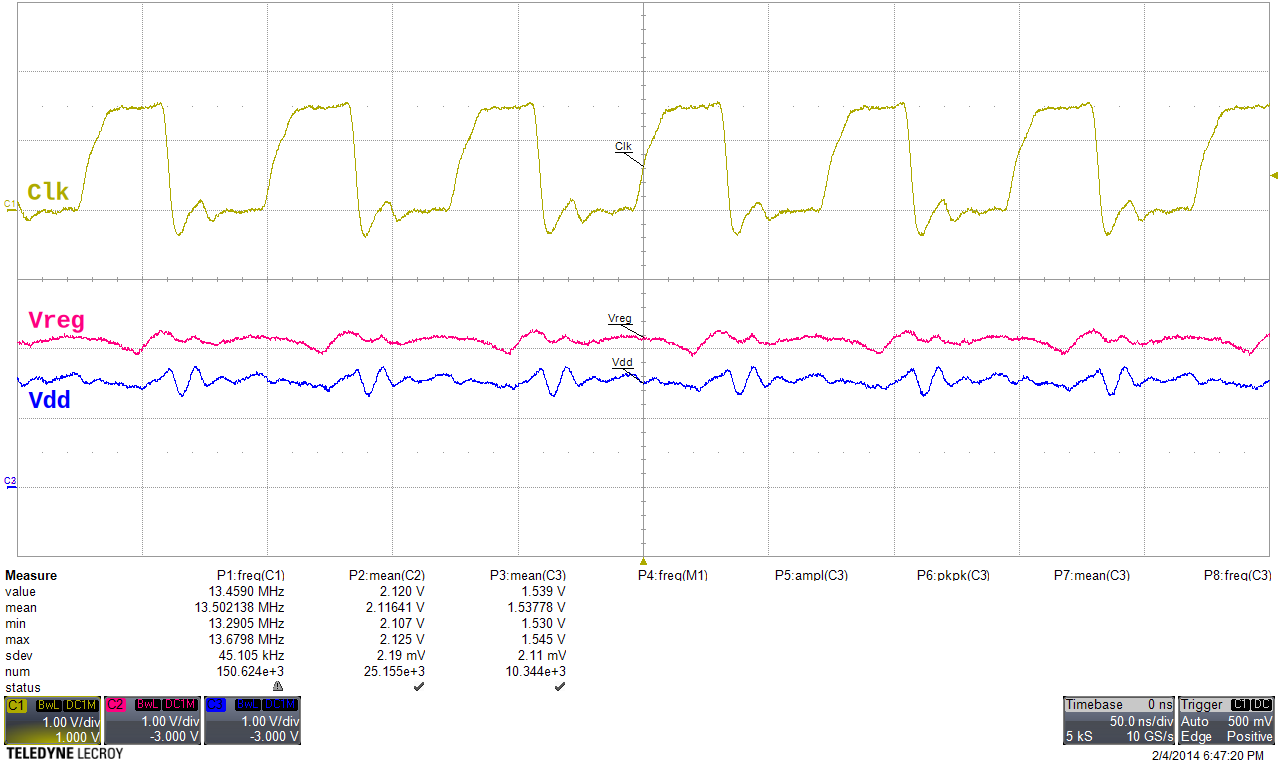
\includegraphics[width=\linewidth]{Captura_ClkVregVdd.pdf}
	\caption{Captura del osciloscopio donde se muestran las señales 
	\emph{Clk}, \emph{Vdd} y \emph{Vreg}.}
	\label{fig:CapturaClkVregVdd}
\end{figure}

En la figura \ref{fig:CapturaPORStartup} se muestra el 
funcionamiento del bloque \emph{Power-on Reset} cuando el dispositivo 
se enciende. El método utilizado para la captura fue el siguiente: con 
las antenas del lector y del transponder separadas a una distancia 
fija, la misma que se uso para la captura de la figura 
\ref{fig:CapturaClkVregVdd}, se encendió la portadora y se disparó el 
osciloscopio con el primer flanco de reloj del chip mientras se 
observaba la salida \emph{POR}. En la figura se ve como la salida del 
bloque \emph{power-on reset} se mantiene en estado alto durante 
\SI{15}{\micro\second}, manteniendo a todo el sistema digital 
\emph{reseteado} y luego liberándolo. No se observaron \emph{glitches} 
en la salida del circuito.

\begin{figure}
	\centering
	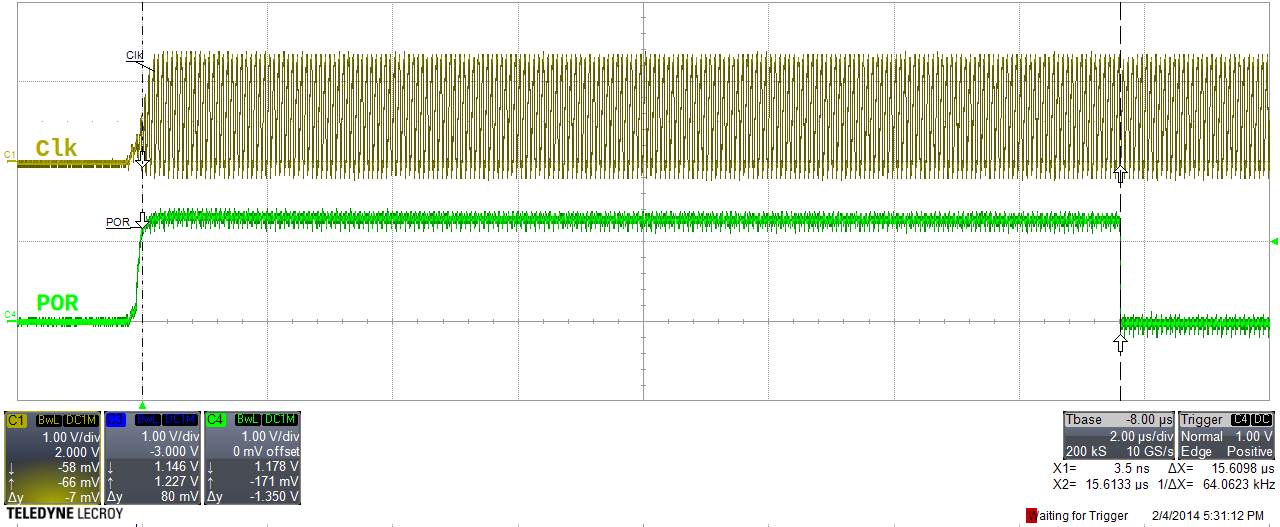
\includegraphics[width=\linewidth]{Captura_POR_Startup.pdf}
	\caption{Captura de la señal \emph{POR} en el 
	arranque del dispositivo. La duración del pulso es de 
	\SI{15}{\micro\second}.}
	\label{fig:CapturaPORStartup}
\end{figure}

Luego se verificó el funcionamiento de la lógica del chip conectando 
el transponder en modo \emph{eco}. Se enviaron diferentes bytes de 
datos, de a uno por vez, comparando la respuesta del transponder con 
el dato enviado y analizando las señale que intervienen en la 
transmisión y recepción de datos. En la secciones siguientes se verá 
en detalle primero la recepción y luego la transmisión a través de 
la interfaz digital.


\subsection{Recepción de datos}

Con el transponder conectado en modo eco, y ubicado a la distancia de 
funcionamiento se envió un byte de datos y se capturaron las señales 
\emph{Clk}, \lstinline{decoder_data}, \lstinline{coded_out} y 
\emph{Pause}. En la figura \ref{fig:CapturaPause} se observa la 
captura realizada, donde se ve como las pausas en la portadora 
interrumpen la señal de reloj y a la vez el detector de pausas cambia 
de estado. 

A través del lector se envió el byte 8'h0F y la portadora 
generada produjo el patrón de reloj de la figura, a partir del cuál es 
válido corroborar la información recibida por el chip. El lector 
envió los datos comenzando por el bit menos significativo como indica 
el estándar, y la señal \lstinline{decoder_data} fue capaz de reconocer
los 8 bits  sin inconvenientes. El reconocimiento de cada bit se 
produce en la cuarta muestra tomada por el módulo 
\lstinline{bit_decoder}, es por eso que \lstinline{decoder_data} 
cambia algunos ciclos de reloj antes de que termine el tiempo del bit.

El estándar requiere que la cantidad de símbolos en <<1>> enviados 
sea impar, es por eso que el lector envió el bit de paridad en `1'. El 
módulo \lstinline{bit_decoder} también leyó correctamente el bit de 
paridad y el símbolo de <<Fin>> de comunicación.

\begin{figure}
	\centering
	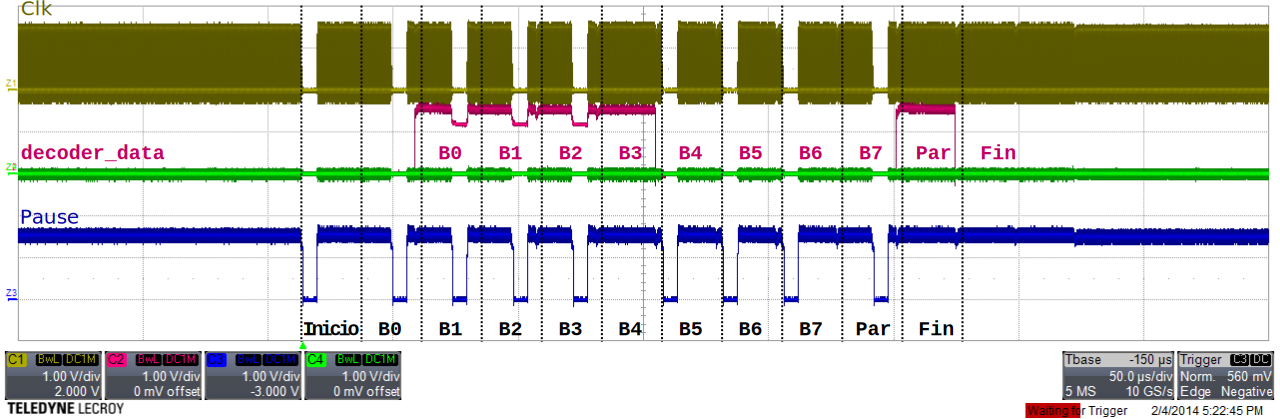
\includegraphics[width=\linewidth]{Captura_eco1byte4_1.pdf}
	\caption{Captura de las señales durante la recepción de datos.}
	\label{fig:CapturaRecepcionDatos}
\end{figure}

Que el módulo digital \lstinline{bit_decoder} haya podido leer la 
información significa que el detector de pausas también funcionó 
correctamente. En la figura \ref{fig:CapturaPause} se observa una 
captura ampliada de la señal \emph{Pause} durante una pausa en la 
portadora. Allí se observa como luego de aproximadamente 
\SI{500}{\nano\second} de comenzada la pausa, la señal pasa al estado 
bajo, indicando que se produjo una pausa y como luego vuelve al nivel 
alto con los primeros ciclos de la portadora. En la figura también se 
observa como se mantiene la tensión de alimentación \emph{Vdd} ---que 
se puede medir en el nivel alto de \emph{Pause}--- en el momento en 
que no se recibe energía.

\begin{figure}
	\centering
	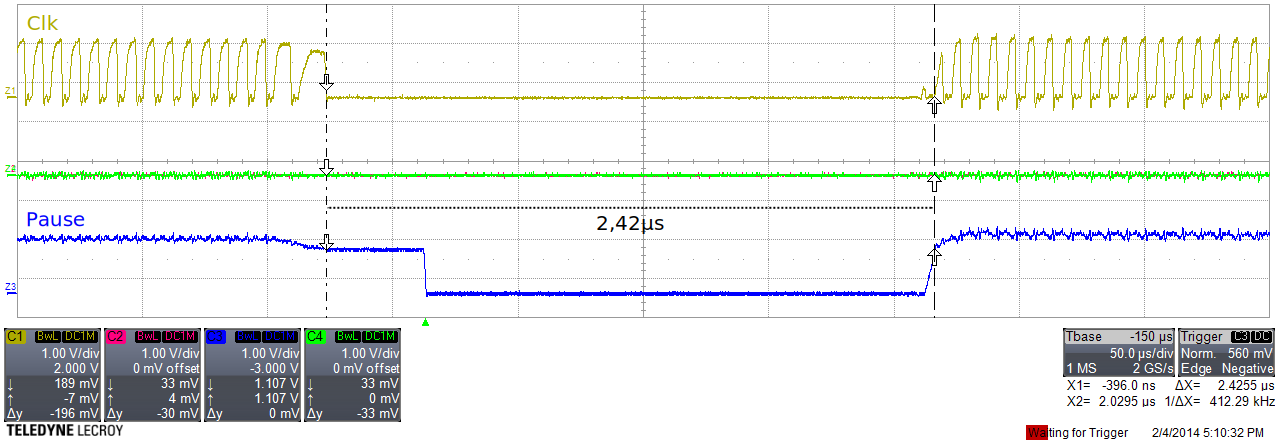
\includegraphics[width=\linewidth]{Captura_Pausa.pdf}
	\caption{Captura de la señal \emph{Pause} durante una pausa en la 
	portadora.}
	\label{fig:CapturaPause}
\end{figure}

En la figura \ref{fig:CapturaRXinterface} se observan las señales a 
la salida del chip, en la interfaz digital de recepción, cuando a 
través del lector se envía el byte 8'h55. El módulo 
\lstinline{Frame Receiver} se encarga de desencapsular la información 
dentro de la trama y por lo tanto a través de la interfaz de salida 
sólo se obtiene el byte de datos. El orden de salida es el mismo que 
el de recepción, es decir, el bit menos significativo se obtiene 
primero y luego los demás. 

Cada bit de datos recibido es presentado a la salida por el módulo 
\lstinline{Frame Receiver}, en la salida \lstinline{rx_bit}, para 
luego generar un pulso de un ciclo de reloj en \lstinline{rx_new_bit}.
Este último pulso informa que existe un nuevo bit en la salida que debe 
ser leído. Al recibir los ocho bits de datos y luego de comprobar que 
el bit de paridad sea correcto, el módulo genera un pulso en 
\lstinline{rx_new_byte}. Finalmente, luego de recibir el símbolo de 
fin de comunicación se genera un pulso por \lstinline{rx_eof} que 
indica el final de la comunicación y que además dispara el contador 
del \emph{Frame Delay Time} (FDT).

\begin{figure}
	\centering
	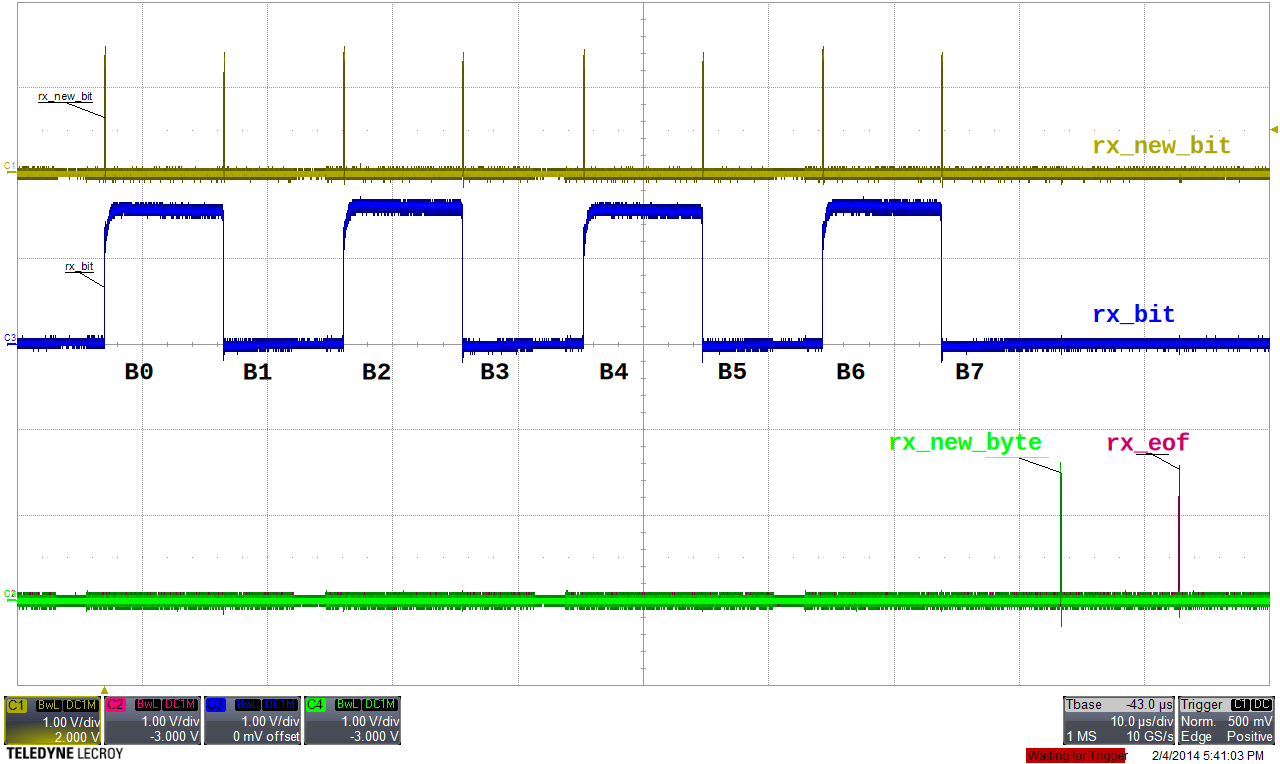
\includegraphics[width=\linewidth]{Captura_RXinterface.pdf}
	\caption{Captura de las señales en la interfaz digital de salida 
	del chip, donde se reciben los datos enviados por el lector.}
	\label{fig:CapturaRXinterface}
\end{figure}


\subsection{Transmisión de Datos}

En la figura \ref{fig:CapturaTXinterface1} se muestra una captura de 
osciloscopio con la secuencia realizada para comprobar el 
funcionamiento del sistema de transmisión de datos del transponder. El 
conexionando de \emph{eco} permitió cargar el buffer de transmisión 
enviando la información directamente con el mismo lector. Al recibir 
los datos el módulo \lstinline{Frame Sender} se encuentra en estado de 
reposo, indicado por la señal \lstinline{tx_ready} en nivel alto. A 
través del lector se envió el valor 8'hAA, que fue recibido por el 
sistema receptor y cargado en el buffer de transmisión, como se 
observa en la figura. Al detectarse 
el símbolo de fin de comunicación enviado por el lector se produce un 
pulso en \lstinline{rx_eof} que se encuentra conectado a 
\lstinline{tx_transmit} y se inicia el proceso de transmisión. El pulso 
no se observa en la figura por la escala utilizada, pero coincide con el 
flanco descendente de \lstinline{tx_ready}. Luego de esperar el tiempo 
FDT \lstinline{coded_out} comienza la modulación de carga. Los datos 
devueltos coinciden con los enviados, respetándose el tiempo de cada 
bit (\SI{9.4}{\micro\second}) y transmitiendo además los bits de 
inicio y paridad.

\begin{figure}
	\centering
	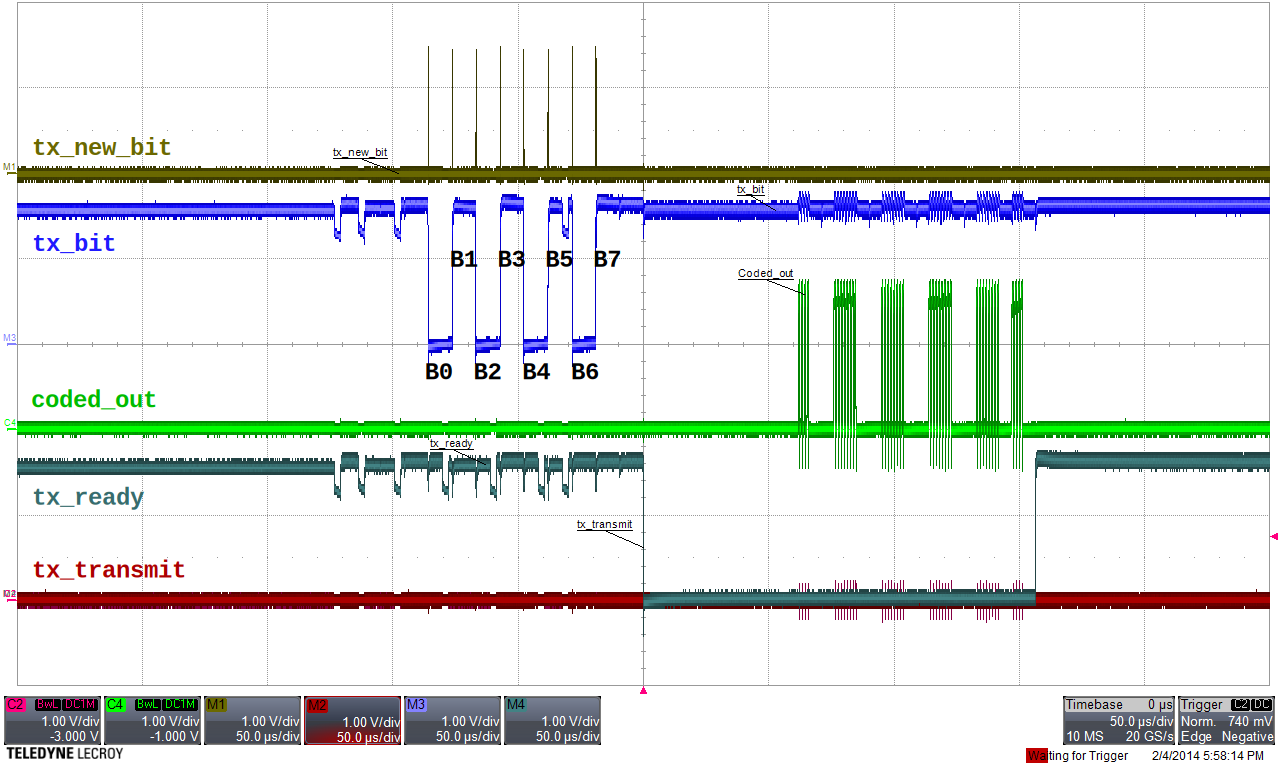
\includegraphics[width=\linewidth]{Captura_TXinterface1.pdf}
	\caption{Captura de las señales de la interfaz digital de 
	transmisión.}%, donde se observa la carga y envío de un byte de datos.}
	\label{fig:CapturaTXinterface1}
\end{figure}

En la figura \ref{fig:CapturaModuladorByte} se muestra una transmisión 
completa de un byte de datos, donde el valor enviado es 8'h0F. La 
transmisión comienza con el símbolo de <<Inicio>>, un `1' lógico, 
luego se envían los ocho bits de datos comenzando por el bit menos 
significativo y finalmente se transmite el bit de paridad. El dato 
enviado contiene una cantidad par de bits en `1', por lo tanto el bit 
de paridad debe ser también `1' para que la transmisión completa sea 
impar. En la captura se ve que el módulo \lstinline{Frame Sender} 
agregó correctamente el bit de paridad.

\begin{figure}
	\centering
	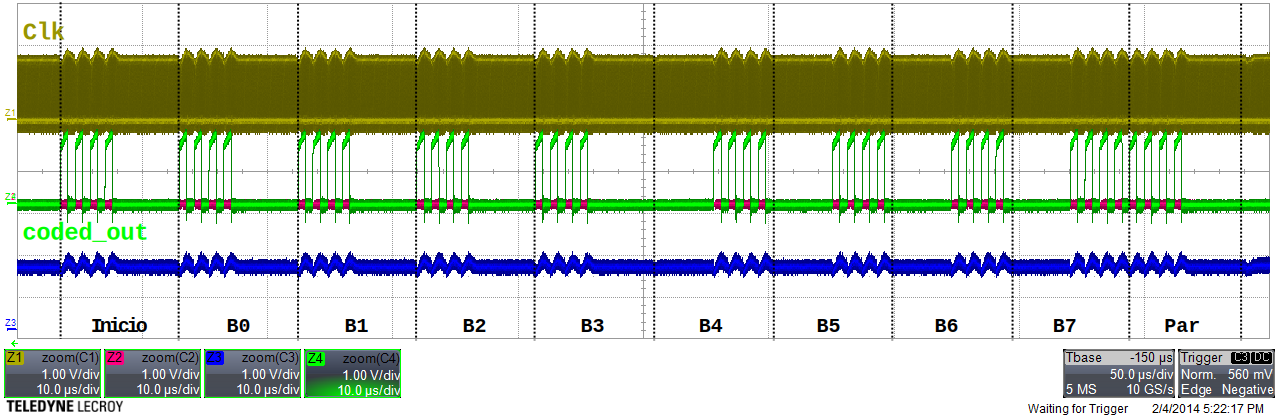
\includegraphics[width=\linewidth]{Captura_TXModulador.pdf}
	\caption{Captura de la salida del modulador en una transmisión 
	completa.}
	\label{fig:CapturaModuladorByte}
\end{figure}


\subsection{Regulador/Limitador de tensión}

Para probar este bloque es necesario contar con un generador de señal 
que sea capaz de alcanzar el campo máximo de 
\SI[per-mode=symbol]{7.5}{\ampere\per\meter}(rms) a una frecuencia de 
\SI{13.56}{\mega\hertz} con la antena indicada en el arreglo dado por 
la norma ISO/IEC 10373--6 (figura \ref{fig:ArregloDeAntenas}). Como no 
se contaba con un generador que tenga esa capacidad, se decidió probar 
el regulador generando el campo con una antena igual a la del 
transponder y colocando ambas antenas lo más cerca posible. La antena 
que actuaba de PCD (lector) fue conectada al generador de funciones 
\emph{Agilent 33220A} y se seteo una amplitud de \SI{20}{\volt}pp, la 
máxima posible.

En la figura \ref{fig:CapturaBmax} se observa el regulador en 
funcionamiento. El transistor de paso deriva corriente a GND y por lo 
tanto la capacidad parásita del nodo \emph{Vreg} llega ahora a 
descargarse, a diferencia de lo que sucedía en la figura 
\ref{fig:CapturaClkVregVdd}, en donde el regulador se encontraba 
inactivo. En este caso la tensión \emph{Vdd} alcanzó un valor medio 
de \SI{2.7}{\volt} y \emph{Vreg} \SI{2.15}{\volt}, este último cercano 
al valor de diseño de \SI{2.5}{\volt}.

\begin{figure}
	\centering
	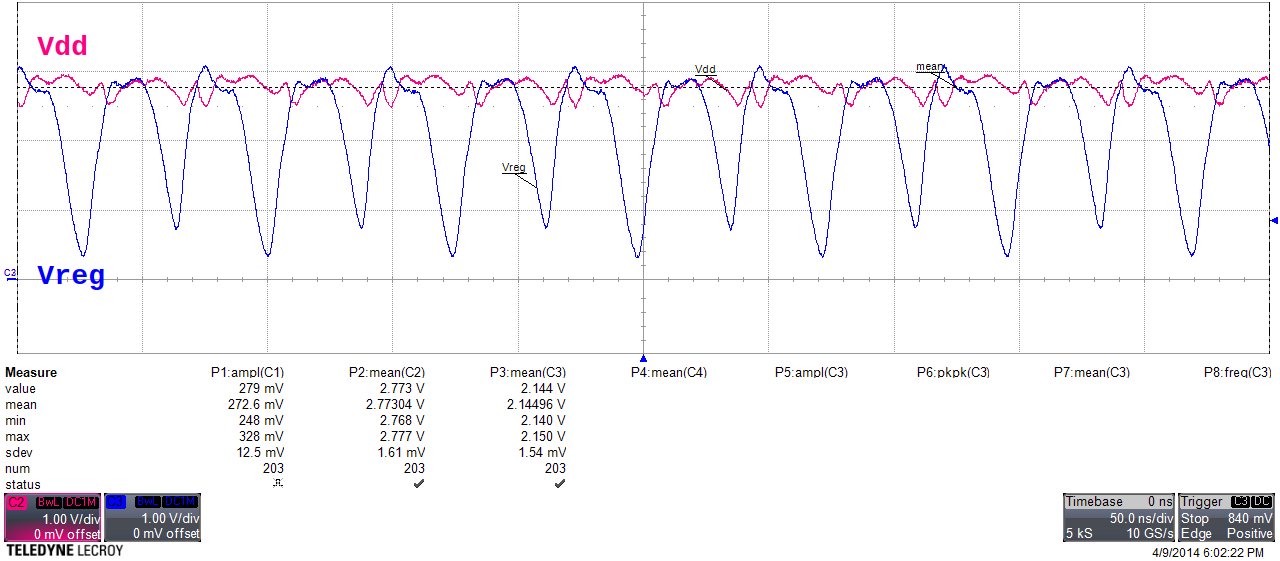
\includegraphics[width=\linewidth]{Captura_PcdAntena8uH_Bmax_20V.pdf}
	\caption{Captura del regulador en funcionamiento con un alto valor 
	de intensidad de campo. La curva azul corresponde a la tensión 
	\(V_{reg}\), cuyo valor medio es \SI{2.14}{\volt}, y la rosada a 
	\(V_{dd}\), con un valor medio de \SI{2.77}{\volt}.}
	\label{fig:CapturaBmax}
\end{figure}


\subsection{Verificación del funcionamiento completo}

Para verificar el funcionamiento de todo el dispositivo se utilizó el 
banco de la figura \ref{fig:FotoSetup} junto con la antena extra para 
espiar la comunicación. Dicha antena fue conectada a la punta 
\(\times10\) del osciloscopio, cuya capacidad de entrada es de 
aproximadamente \SI{15}{\pico\farad}, lo que formó un circuito tanque 
LC que mejoró la recepción de la señal. El transponder fue conectado 
en modo \emph{eco} de forma tal de tener todos los bloques internos 
en funcionamiento.

En la figura \ref{fig:CapturaSniffer} se muestra una captura realizada 
con la antena espía. Allí puede verse la trama transmitida por el 
lector, que contiene el byte 8'hA5 y luego la respuesta del 
transponder modulando la portadora según lo indica el estándar y 
respondiendo con la misma información. Además se ve como el 
transponder envía en la trama el bit de paridad correcto.

\begin{figure}
	\centering
	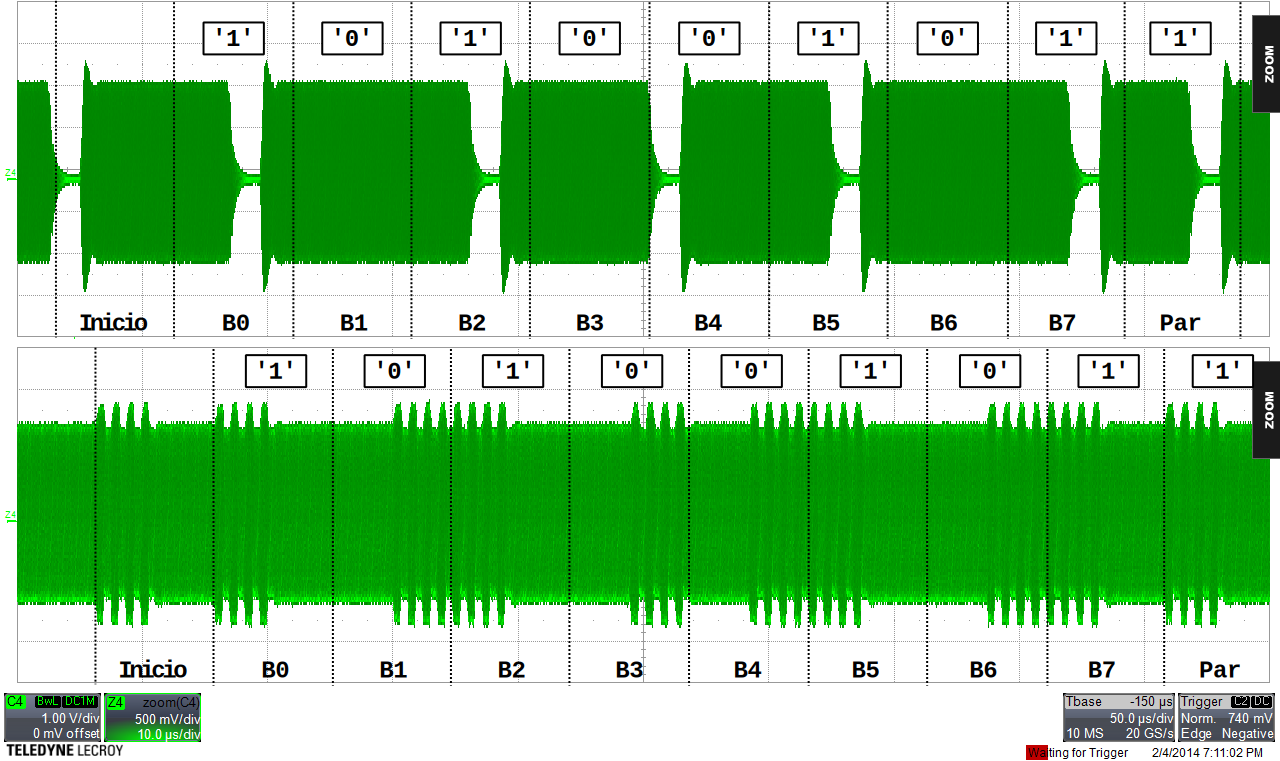
\includegraphics[width=\linewidth]{Captura_sniffer_byteEcho.pdf}
	\caption{Captura de la comunicación entre lector y transponder con 
	la antena espía. El gráfico superior corresponde a una trama de un 
	byte enviada por el lector, mientras que el inferior corresponde 
	a la respuesta de eco del transponder.}
	\label{fig:CapturaSniffer}
\end{figure}

Finalmente, se desarrolló un pequeño programa en lenguaje \emph{Python} 
para controlar el lector y enviar los bytes de 8'h00 a 8h'FF, leer 
las respuestas del transponder y comparar la información enviada con la 
recibida. Como se dijo antes, el lector utiliza un circuito integrado 
comercial de \emph{Texas Instruments} que contiene una implementación 
del protocolo ISO/IEC 14443-A utilizada alrededor del mundo. El 
programa de prueba envía al lector sólo la información que se debe 
transmitir, y es el lector el que encapsula esa información en una 
trama estándar y la envía a través de la antena. Lo mismo sucede 
durante la recepción, el lector recibe una trama que \emph{debe} 
cumplir con el estándar y presenta la información al programa de 
prueba.

La prueba del eco con los 256 bytes de datos, enviados y recibidos de 
a uno por vez, fue todo un éxito, dando como resultado una tasa de 
pérdida de 0\%, es decir, todos los bytes fueron respondidos 
correctamente por el circuito integrado. 
